\documentclass[11pt,a4paper]{article}

\usepackage[utf8]{inputenc}
\usepackage[T1]{fontenc}
\usepackage[brazilian]{babel}
\usepackage{geometry}
\geometry{margin=2.3cm}
\usepackage{graphicx}
\usepackage{booktabs}
\usepackage{longtable}
\usepackage{array}
\usepackage{xcolor}
\usepackage{hyperref}
\hypersetup{
  colorlinks=true,
  linkcolor=blue!50!black,
  citecolor=blue!50!black,
  urlcolor=blue!50!black,
}
\usepackage{listings}
\usepackage{enumitem}
\usepackage{fancyhdr}
\usepackage{titlesec}
\usepackage{tcolorbox}
\tcbuselibrary{skins,breakable}

\definecolor{codebg}{RGB}{245,245,245}
\definecolor{codeframe}{RGB}{200,200,200}

\lstdefinestyle{shell}{
  backgroundcolor=\color{codebg},
  basicstyle=\ttfamily\small,
  breaklines=true,
  frame=single,
  rulecolor=\color{codeframe},
  columns=fullflexible,
  keepspaces=true,
  showstringspaces=false,
}
\lstset{style=shell}

\newtcolorbox{stepbox}[1]{
  colback=green!5!white,
  colframe=green!40!black,
  fonttitle=\bfseries,
  title=#1,
  breakable,
}
\newtcolorbox{warningbox}[1]{
  colback=orange!5!white,
  colframe=orange!60!black,
  fonttitle=\bfseries,
  title=#1,
  breakable,
}
\newtcolorbox{infobox}[1]{
  colback=blue!5!white,
  colframe=blue!40!black,
  fonttitle=\bfseries,
  title=#1,
  breakable,
}

\setlength{\headheight}{14pt}
\pagestyle{fancy}
\fancyhf{}
\rhead{\small Guia final de execução — IC}
\lhead{\small Injeção de contexto no preditor de intenção}
\rfoot{\thepage}

\titleformat{\section}{\normalfont\Large\bfseries}{\thesection}{1em}{}
\titleformat{\subsection}{\normalfont\large\bfseries}{\thesubsection}{1em}{}

\title{\textbf{Guia Final de Execução} \\[0.2cm]
\large Injeção de Contexto de Tarefa no Preditor de Intenção}
\author{Marcos Kalile \\ \small Projeto PIBIC/CNPq --- IME/LIARC \\ \small Orientador: Prof. Hebert Azevedo-Sá}
\date{8 de julho de 2026}

\begin{document}

\maketitle

\begin{infobox}{Leia isto primeiro}
Todo o código (OS-1 a OS-7) já está pronto e testado (16/16 testes
automatizados). O que falta é executar 4 blocos, nesta ordem:
\textbf{(1) gravar e anotar sessões, (2) consolidar 3 datasets,
(3) treinar V0/V1/V2, (4) gerar tabela e figuras finais.}
Este guia é um roteiro de execução, não uma justificativa de decisões de
projeto (essas já estão no \texttt{ROADMAP\_IC.pdf}). Cada seção abaixo diz
exatamente o que fazer e qual comando rodar.
\end{infobox}

\tableofcontents
\newpage

% =============================================================
\section{Visão geral: os 4 blocos}
% =============================================================

\begin{center}
\begin{tabular}{@{}p{1cm}p{4.3cm}p{6cm}p{2.8cm}@{}}
\toprule
\textbf{Bloco} & \textbf{O que fazer} & \textbf{Ferramenta} & \textbf{Tempo estimado} \\
\midrule
1 & Gravar e anotar 12 sessões (Seção~\ref{sec:dataset}) & \texttt{capture\_session}, \texttt{annotate\_pkl} & 1--2 dias \\
2 & Consolidar 3 datasets de contexto (Seção~\ref{sec:consolidacao}) & \texttt{build\_json} & 15 min \\
3 & Treinar V0, V1, V2 (Seção~\ref{sec:treino}) & \texttt{train\_finetune.py} & algumas horas (CPU) \\
4 & Gerar tabela e matrizes de confusão (Seção~\ref{sec:matrizes}) & \texttt{aggregate\_results.py} & 5 min \\
\bottomrule
\end{tabular}
\end{center}

Ambiente usado em todos os comandos: conda \texttt{hrc}
(\texttt{source /home/marcos-kalile/anaconda3/bin/activate hrc}). Coleta e
consolidação rodam em \texttt{hrc-data-collection/}; treino e agregação
rodam em \texttt{hrc-finetune/}.

% =============================================================
\section{Bloco 1 --- Gravar e anotar as sessões}
\label{sec:dataset}
% =============================================================

\subsection{Bancada (montar uma vez, não mexer mais)}

\begin{itemize}
  \item 8 conectores, 12 parafusos, 4 rodas, 8 tubos curtos ($\sim$12\,cm), 4 tubos longos ($\sim$25\,cm);
  \item conectores à direita; parafusos à esquerda perto; rodas à esquerda atrás dos parafusos; gabarito ao centro; marca de repouso na borda;
  \item 40--50\,cm entre zonas.
\end{itemize}

\begin{warningbox}{Não mude entre sessões}
Câmera, posição das zonas, cadeira, iluminação: fixas do início ao fim das
12 sessões. Só variam ordem de pegas, ritmo e postura inicial.
\end{warningbox}

\subsection{As 6 rotas canônicas}
\label{sec:rotas-canonicas}

As rotas abaixo vêm do documento \texttt{Rotas\_e\_Vetor\_de\_Contexto.pdf}
(política \texttt{proxy\_graph}, a mesma que \texttt{plan\_sim.py} já usa em
produção) e foram validadas contra o simulador --- os passos e o contexto
7D exibidos por rota já são a saída real de \texttt{plan\_sim.py}, não uma
estimativa. Use-as como roteiro de gravação.

\begin{longtable}{p{1cm}p{3.2cm}p{8cm}p{1.3cm}}
\toprule
\textbf{Rota} & \textbf{Papel} & \textbf{Sequência} & \textbf{Passos} \\
\midrule
\endhead
R01 & Tarefa completa (canônica) & \texttt{bottom} $\to$ \texttt{four\_tubes} $\to$ \texttt{top} $\to$ \texttt{wheels}. Fecha com contexto \texttt{[1000\,|\,1.00,1.00,1.00]}. Esta é a rota de referência. & 29 \\
R02 & Estágio \texttt{bottom} isolado & Só a primeira parte de R01 (4 conectores + 4 parafusos de \texttt{bottom}), sem prosseguir. Rota mínima de validação. & 8 \\
R03 & \texttt{bottom} $\to$ \texttt{four\_tubes} & Prefixo de R01 até o fim de \texttt{four\_tubes}, sem \texttt{top}/\texttt{wheels}. & 17 \\
R04 & Retomada via \texttt{--stageI\_done} & Começa direto em \texttt{four\_tubes} (bottom já assumido pronto), segue \texttt{top} $\to$ \texttt{wheels}. Usa o preset de retomada do simulador. & 21 \\
R05 & Completa com \texttt{no\_action} intercalado & Mesma sequência de R01, mas com pausas de \texttt{no\_action} inseridas em pontos de contexto igual (engorda a classe \texttt{no\_action} sem inventar contexto novo). & 32 \\
R06 & Ordem alternativa & \texttt{bottom} $\to$ \texttt{top} $\to$ \texttt{four\_tubes} $\to$ \texttt{wheels} (troca a posição de \texttt{top} e \texttt{four\_tubes} em relação a R01). Também válida no grafo. & 29 \\
\bottomrule
\end{longtable}

\begin{infobox}{Como usar as 6 rotas para montar as sessões}
\begin{itemize}[leftmargin=1.5em]
\item \textbf{R01 primeiro, sempre}: grave e anote só ela, rode o Bloco 2
com \texttt{--allow-empty-split} para validar a cadeia inteira antes de
investir nas demais.
\item \textbf{Diversidade estrutural} (muda a sequência de estágios,
robustece o vetor de contexto contra viés de ordem): alterne R01 e R06 nas
repetições de treino.
\item \textbf{Diversidade de trajetória} (mesmo grafo, mesmo contexto,
esqueleto diferente): use R05 para gerar exemplos de \texttt{no\_action}
com o mesmo par (contexto, próxima intenção) que R01, variando só a
execução física (pausas, micro-variações de postura, ritmo).
\item \textbf{R02/R03/R04 são rotas curtas}, úteis para engordar classes
específicas (\texttt{bottom} isolado, transição para \texttt{four\_tubes},
retomada) sem repetir a tarefa inteira --- gravação mais rápida quando
faltar janela de uma classe pontual.
\item Recomendação do documento de rotas: execute R01/R06 com variação
natural (ritmo, postura) e \textbf{repita cada uma 8--12 vezes} para
densificar amostras por par (intenção, estágio). Isso substitui a ideia de
"12 sessões distintas com rótulos artificiais" por "poucas rotas bem
definidas, repetidas com variação natural".
\end{itemize}
\end{infobox}

\subsection{Quantas sessões gravar}
\label{sec:ordem-sessoes}

\begin{center}
\begin{tabular}{@{}p{2.5cm}p{9cm}p{2cm}@{}}
\toprule
\textbf{Sessões} & \textbf{O que gravar} & \textbf{Split} \\
\midrule
1.ª & R01 (piloto --- valida a cadeia antes de continuar) & treino \\
2.ª--5.ª & Alterne R01/R06 (2 de cada), ritmo e postura naturais entre repetições & treino \\
6.ª--8.ª & R05 (completa com \texttt{no\_action} intercalado), variando ritmo & treino \\
9.ª & R02, R03 ou R04 --- só a que estiver mais fraca após o Bloco 2 & treino \\
\textbf{10.ª} & \textbf{R01} completa, ritmo normal. Sessão \textbf{inteira} reservada para teste --- não editar depois de gravar. & \textbf{teste} \\
\textbf{11.ª} & \textbf{R06} completa, ritmo normal. Segunda sessão de teste. & \textbf{teste} \\
12.ª (buffer) & \textbf{Só grave se} o relatório do Bloco 2 (Seção~\ref{sec:sanidade}) mostrar alguma classe com $<$120 janelas. Repita a rota que cobre essa classe. & a definir \\
\bottomrule
\end{tabular}
\end{center}

\subsection{Como gravar cada sessão}

Repita este bloco de comandos para cada uma das 11--12 sessões da tabela
acima. Troque \texttt{--script-id} pela rota da linha atual (\texttt{R01},
\texttt{R06}, \texttt{R05}, etc.).

\begin{lstlisting}[language=bash]
cd /home/marcos-kalile/hrc-data-collection
source .venv/bin/activate

# ID sugerido automaticamente (formato SNN_YYYYMMDD)
python -m datacol.capture_session --suggest-session-id

# Gravar (troque --script-id pela rota desta sessao: R01, R06, R05, ...)
python -m datacol.capture_session \
  --participant P01 --script-id R01 \
  --camera-model "Intelbras WCI 1080p" --camera-distance-m 2.2 \
  --width 1920 --height 1080 --fps 30

# Validar logo em seguida
python -m datacol.capture_session --validate-session sessions/<ID_GERADO>
\end{lstlisting}

Regra de execução do gesto, sempre: parado no repouso $\to$ mão até a zona
$\to$ pega e deposita $\to$ volta ao repouso $\to$ pausa breve $\to$ próximo
gesto. Nunca encadeie dois gestos sem passar pelo repouso. Varie o ritmo e a
postura de repouso naturalmente entre repetições da mesma rota (isso já
cobre a diversidade de trajetória sem precisar de rótulos extras de
"rápido"/"lento").

\subsection{Como anotar cada sessão}

Anote logo depois de gravar (não acumule). Para cada sessão:

\begin{lstlisting}[language=bash]
python -m datacol.annotate_pkl sessions/<ID_GERADO>
\end{lstlisting}

Por gesto: \texttt{Espaço} pausa/toca $\to$ \texttt{b} no primeiro quadro do
gesto $\to$ navegue até o último quadro $\to$ tecla da classe
(\texttt{1}=conectores, \texttt{2}=parafusos, \texttt{3}=rodas,
\texttt{i}=ignore). No bloco dos 4 tubos curtos de \texttt{four\_tubes}:
marque tudo como \texttt{ignore}, volte ao primeiro quadro do bloco e
pressione \texttt{f}. Pressione \texttt{s} para salvar --- o programa recusa
se houver lacuna ou sobreposição.

Contagem esperada por sessão R01/R06 (tarefa completa): 8
\texttt{get\_connectors}, 12 \texttt{get\_screws}, 4 \texttt{get\_wheels}, 9
\texttt{ignore}, 1 evento \texttt{begin\_four\_tubes}. Rotas curtas (R02,
R03, R04) têm contagens proporcionalmente menores --- confira contra a
coluna "Passos" da Seção~\ref{sec:rotas-canonicas} (cada passo da tabela é
uma ação/intenção; \texttt{no\_action} e \texttt{ignore} não entram nessa
contagem).

\textbf{Toda sessão com \texttt{four\_tubes}} (R01, R03, R04, R05, R06):
antes de consolidar, rode
\texttt{python -m datacol.context\_replay sessions/<ID> --context-dim 7} e
confirme visualmente que o estágio muda no quadro certo.

% =============================================================
\section{Bloco 2 --- Consolidar os 3 datasets}
\label{sec:consolidacao}
% =============================================================

Depois de anotar todas as sessões, gere os três JSONs (\texttt{context\_dim}
0, 7, 10) \textbf{numa única rodada de comandos}, sempre com os mesmos IDs
de teste:

\begin{lstlisting}[language=bash]
cd /home/marcos-kalile/hrc-data-collection
source .venv/bin/activate

for dim in 0 7 10; do
  python -m datacol.build_json \
    --sessions-root sessions \
    --output datasets/v1/dataset_dim${dim}.json \
    --report datasets/v1/report_classes_dim${dim}.md \
    --test-session <ID_SESSAO_10_R01> \
    --test-session <ID_SESSAO_11_R06> \
    --context-dim ${dim} \
    --window-size 5
done
\end{lstlisting}

Troque \texttt{<ID\_SESSAO\_10\_R01>}/\texttt{<ID\_SESSAO\_11\_R06>} pelos
IDs reais das duas sessões de teste (10.ª e 11.ª da
Seção~\ref{sec:ordem-sessoes}, formato \texttt{SNN\_YYYYMMDD}).

\subsection{Checklist de sanidade (2 minutos, não pule)}
\label{sec:sanidade}

Abra os três \texttt{report\_classes\_dim*.md} e confira:

\begin{stepbox}{Confirme antes de treinar}
\begin{enumerate}[leftmargin=1.5em]
  \item Contagem de janelas por classe é \textbf{igual} nos três relatórios.
  \item Nenhuma classe com zero janelas em nenhum split.
  \item Cada classe com $\geq$120 janelas (treino+teste). Se faltar $\to$ grave R12 focado nessa classe e repita o Bloco 2.
  \item \texttt{no\_action} não deve passar de $\sim$50\% do total.
\end{enumerate}
\end{stepbox}

% =============================================================
\section{Bloco 3 --- Treinar V0, V1, V2}
\label{sec:treino}
% =============================================================

\begin{center}
\begin{tabular}{@{}p{1.3cm}p{5.5cm}p{7cm}@{}}
\toprule
\textbf{Variante} & \textbf{O que é} & \textbf{Para que serve} \\
\midrule
V0 & Checkpoint original, sem treinar & mede o gap webcam vs.\ dados originais \\
V1 & Fine-tune sem contexto & mede o ganho só do fine-tuning \\
V2 & Fine-tune com contexto, partindo de V1 & \textbf{resultado principal}: delta V2$-$V1 \\
\bottomrule
\end{tabular}
\end{center}

\begin{warningbox}{Regra fixa}
Treine nesta ordem: V0 $\to$ V1 $\to$ V2. V2 sempre parte do checkpoint de
V1 (nunca de V0), e cada seed de V2 parte do \textbf{mesmo número de seed}
em V1 (seed 0 de V2 vem do seed 0 de V1, etc.).
\end{warningbox}

\subsection{Comandos, na ordem}

\begin{lstlisting}[language=bash]
cd /home/marcos-kalile/hrc-finetune
source /home/marcos-kalile/anaconda3/bin/activate hrc

CKPT=/home/marcos-kalile/IC_Kalile_Intention_Prediction_HRC/traj_intention/checkpoints/seq5_pred5_epoch40_whole_pkl_final_intention_nomaskTrue.pth
DS=/home/marcos-kalile/hrc-data-collection/datasets/v1

# --- V0: so avalia o checkpoint original ---
python train_finetune.py --variant V0 \
  --dataset $DS/dataset_dim0.json --context-dim 0 \
  --init-checkpoint $CKPT --out-dir runs/V0

# --- V1: fine-tune sem contexto, 3 sementes ---
python train_finetune.py --variant V1 \
  --dataset $DS/dataset_dim0.json --context-dim 0 \
  --init-checkpoint $CKPT --seeds 0 1 2 \
  --epochs 10 --lr 1e-4 --batch-size 32 --out-dir runs/V1

# --- V2: fine-tune com contexto 7D, partindo de V1 (mesma seed) ---
python train_finetune.py --variant V2 \
  --dataset $DS/dataset_dim7.json --context-dim 7 \
  --init-checkpoint-per-seed runs/V1/seed0/checkpoint.pth \
                              runs/V1/seed1/checkpoint.pth \
                              runs/V1/seed2/checkpoint.pth \
  --seeds 0 1 2 --epochs 10 --freeze-epochs 4 \
  --lr 1e-4 --context-lr 1e-3 --batch-size 32 --out-dir runs/V2_dim7

# --- V2 (10D), so se sobrar tempo: ablacao opcional ---
python train_finetune.py --variant V2 \
  --dataset $DS/dataset_dim10.json --context-dim 10 \
  --init-checkpoint-per-seed runs/V1/seed0/checkpoint.pth \
                              runs/V1/seed1/checkpoint.pth \
                              runs/V1/seed2/checkpoint.pth \
  --seeds 0 1 2 --epochs 10 --freeze-epochs 4 \
  --lr 1e-4 --context-lr 1e-3 --batch-size 32 --out-dir runs/V2_dim10
\end{lstlisting}

Cada rodada grava checkpoint + \texttt{metrics.json} por seed, mais um
\texttt{summary.json} com média $\pm$ desvio-padrão. Se o dataset final
tiver poucas janelas por classe, baixe \texttt{--batch-size} para 8--16.

\begin{infobox}{Por que não há perda de trajetória}
O treino original usa duas perdas (classificação + regressão de
trajetória). O dataset novo (\texttt{build\_json.py}) só grava a janela de
entrada e o rótulo — não o alvo de trajetória futura — então
\texttt{train\_finetune.py} treina só com a perda de classificação. Isso é
proposital: o objetivo é isolar o efeito do contexto na classificação, não
reproduzir a tarefa de trajetória do artigo original.
\end{infobox}

% =============================================================
\section{Bloco 4 --- Tabela final e matrizes de confusão}
\label{sec:matrizes}
% =============================================================

\begin{lstlisting}[language=bash]
cd /home/marcos-kalile/hrc-finetune
source /home/marcos-kalile/anaconda3/bin/activate hrc
pip install scikit-learn matplotlib -q

python reports/scripts/aggregate_results.py \
  --runs-root runs --out-dir results
\end{lstlisting}

Gera \texttt{results/ablation\_table.md} (tabela V0/V1/V2 com acurácia, ECE
e o delta V2$-$V1) e \texttt{results/confusion\_matrices.png} (uma matriz
por variante, lado a lado).

\subsection{Exemplo de figura (dados sintéticos, só para conferir o formato)}

\begin{figure}[htbp]
\centering
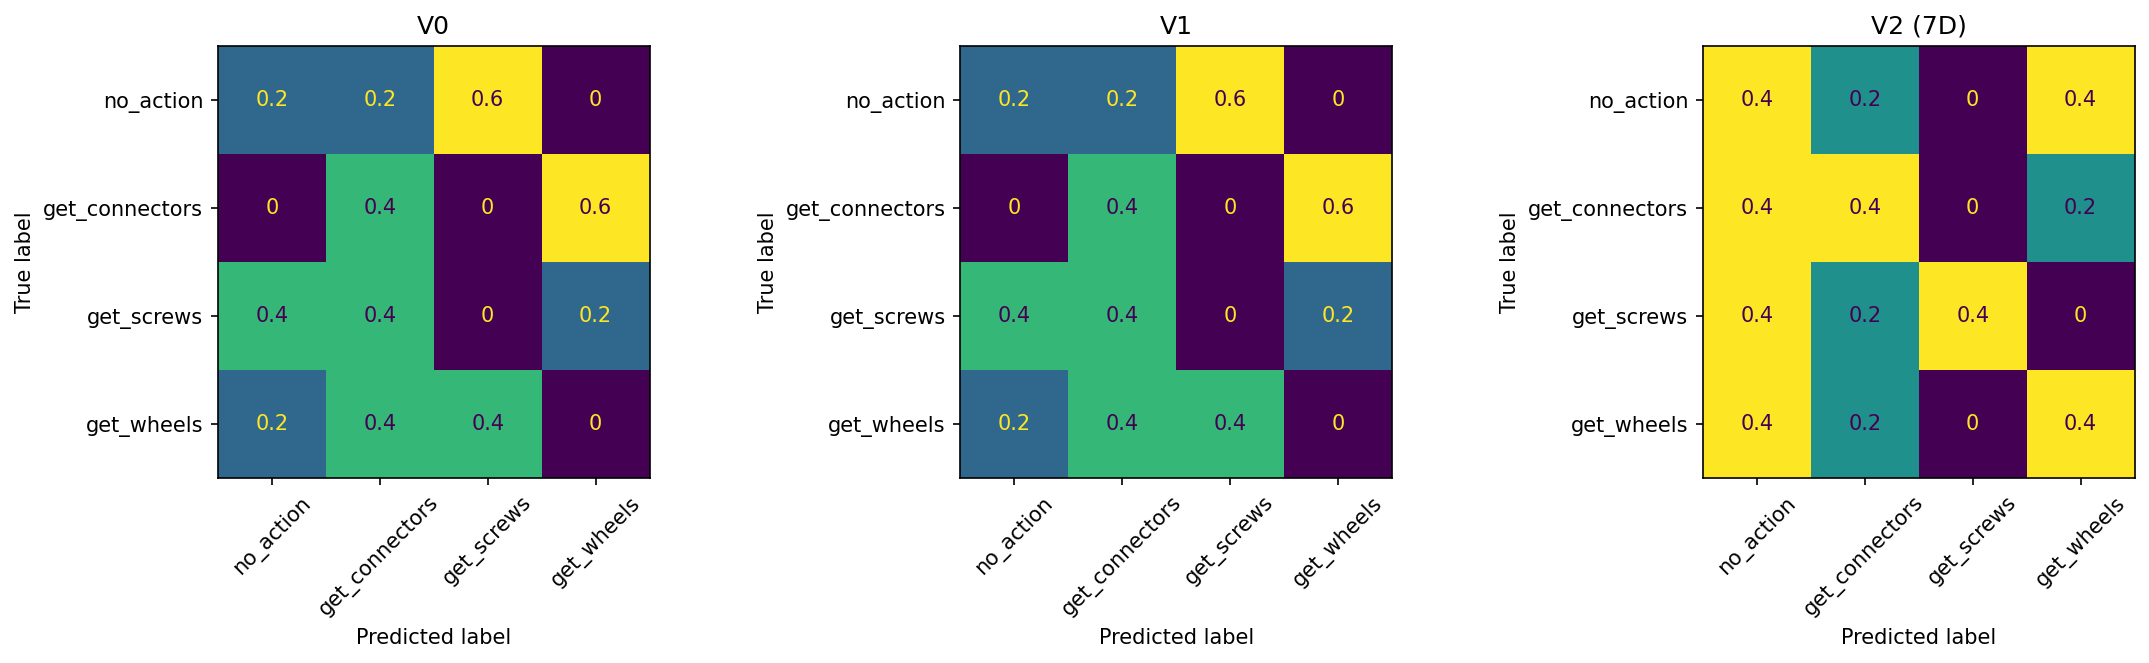
\includegraphics[width=\textwidth]{figures/confusion_matrices_example.png}
\caption{Formato esperado da figura final — substitua rodando o script acima
com \texttt{runs/} real.}
\label{fig:cm-exemplo}
\end{figure}

\subsection{Como ler o resultado}

\begin{itemize}[leftmargin=1.5em]
  \item Diagonal da matriz = acurácia por classe (cada linha soma 1).
  \item V0 $\to$ V1: melhora mede a adaptação de domínio (fine-tuning puro).
  \item V1 $\to$ V2: melhora adicional é o efeito do contexto --- \textbf{este é o resultado central do artigo}.
  \item Metas de referência do roadmap: top-1 $\geq$ 70\% e ECE $<$ 0,08 em V2. Se não bater, o resultado ainda é publicável: o que importa é o delta V2$-$V1, não o valor absoluto.
\end{itemize}

% =============================================================
\section{Checklist único}
% =============================================================

\begin{stepbox}{Do início ao fim}
\begin{enumerate}[leftmargin=1.5em]
  \item Gravar + anotar a 1.ª sessão (rota R01). Rodar Bloco 2 com \texttt{--allow-empty-split} para validar a cadeia.
  \item Gravar + anotar as demais 9--10 sessões de treino (rotas R01/R06/R05/R02/R03/R04 conforme a Seção~\ref{sec:ordem-sessoes}), anotando cada uma logo após gravar.
  \item Gravar + anotar as 2 sessões de teste (rotas R01 e R06, ritmo normal, sessão inteira reservada).
  \item Rodar \texttt{context\_replay} em toda sessão com \texttt{four\_tubes} (R01, R03, R04, R05, R06).
  \item Rodar Bloco 2 completo (3 datasets) com os IDs reais das 2 sessões de teste.
  \item Checar os 3 relatórios de classes (Seção~\ref{sec:sanidade}). Se faltar janela, gravar a 12.ª sessão buffer e repetir.
  \item Rodar V0, depois V1 (3 sementes), depois V2 7D (3 sementes pareadas). V2 10D se sobrar tempo.
  \item Rodar \texttt{aggregate\_results.py}.
  \item Escrever a seção de resultados do artigo com \texttt{ablation\_table.md} e \texttt{confusion\_matrices.png}.
\end{enumerate}
\end{stepbox}

\begin{infobox}{Onde está cada arquivo}
\begin{itemize}[leftmargin=1.5em]
\item Coleta/anotação/consolidação: \texttt{\small hrc-data-collection/src/datacol/}
\item Treino e inferência: \texttt{\small hrc-finetune/\{train\_finetune,DLinear,predict\}.py}
\item Testes: \texttt{\small hrc-finetune/tests/}
\item Agregação de resultados: \texttt{\small hrc-finetune/reports/scripts/aggregate\_results.py}
\item Este guia: \texttt{\small hrc-finetune/reports/relatorio\_final\_ic.tex}
\end{itemize}
\end{infobox}

\appendix

% =============================================================
\section{Rotas detalhadas, passo a passo}
\label{ap:rotas}
% =============================================================

Este apêndice traz o roteiro completo de cada rota, extraído de
\texttt{Rotas\_e\_Vetor\_de\_Contexto.pdf} (saída real de
\texttt{plan\_sim.py}, política \texttt{proxy\_graph}). Use como guia
literal de gravação: cada linha é um gesto a executar na bancada, na ordem
exata. \textbf{Contexto 7D} = one-hot de estágio
\texttt{[none,bottom,four\_tubes,top]} $\parallel$ conectores/8,
parafusos/12, rodas/4.

Convenções das tabelas: \textbf{Gesto} é o que fazer com as mãos (classe a
rotular depois, ou \textit{ignore}/transição); \textbf{Estágio} é o estágio
ativo após o gesto; \textbf{Parafusos} mostra a contagem acumulada por
estágio no formato \texttt{b}=bottom, \texttt{ft}=four\_tubes, \texttt{t}=top
(ex.\ \texttt{b2 ft0 t0} = 2 parafusos em bottom, 0 nos demais).

\subsection{R01 --- Tarefa completa (rota canônica)}
\label{ap:r01}

\textbf{Ordem:} \texttt{bottom} $\to$ \texttt{four\_tubes} $\to$
\texttt{top} $\to$ \texttt{wheels}. \textbf{29 passos.} \textbf{Contexto
final:} \texttt{[1000\,|\,1.00,1.00,1.00]} (tudo completo, sem estágio
ativo).

\begin{longtable}{p{0.6cm}p{3.1cm}p{2.6cm}p{2.3cm}p{5.5cm}}
\toprule
\textbf{\#} & \textbf{Gesto} & \textbf{Estágio} & \textbf{Parafusos} & \textbf{Contexto 7D após o gesto} \\
\midrule
\endhead
1--4 & \texttt{get\_connectors} $\times$4 (2 curtos + 2 longos) em \texttt{bottom} & bottom $\to$ none & b0 ft0 t0 & sobe de \texttt{[0,1,0,0\,|\,0.12,0,0]} até \texttt{[1,0,0,0\,|\,0.50,0,0]} \\
5--8 & \texttt{get\_screws} $\times$4 em \texttt{bottom} & none & b1$\to$b4 ft0 t0 & parafusos sobe 0.08 por vez, de 0.42 até \texttt{[1000\,|\,0.50,0.33,0]} \\
9 & \textit{begin\_four\_tubes} (transição, marcar \texttt{f} na anotação) & four\_tubes & b4 ft0 t0 & \texttt{[0,0,1,0\,|\,0.50,0.33,0]} \\
10--13 & \texttt{short} $\times$4 (colocação manual dos 4 tubos curtos, \textit{ignore} na anotação) & four\_tubes $\to$ none & b4 ft0 t0 & sobe conectores até \texttt{[1000\,|\,1.00,0.33,0]} \\
14--17 & \texttt{get\_screws} $\times$4 em \texttt{four\_tubes} & none & b4 ft1$\to$ft4 t0 & parafusos sobe até \texttt{[1000\,|\,1.00,0.67,0]} \\
18--21 & \texttt{get\_connectors} $\times$4 (2 curtos + 2 longos) em \texttt{top} & top $\to$ none & b4 ft4 t0 & \texttt{[0,0,0,1\,|\,1.00,0.67,0]} durante, volta a \texttt{[1000\,|...]} ao fechar \\
22--25 & \texttt{get\_screws} $\times$4 em \texttt{top} & none & b4 ft4 t1$\to$t4 & parafusos sobe até \texttt{[1000\,|\,1.00,1.00,0]} \\
26--29 & \texttt{get\_wheels} $\times$4 (rodas) & none & b4 ft4 t4 & rodas sobe 0.25 por vez até \texttt{[1000\,|\,1.00,1.00,1.00]} \\
\bottomrule
\end{longtable}

\textbf{Ao anotar:} 8 intervalos \texttt{get\_connectors}, 12
\texttt{get\_screws}, 4 \texttt{get\_wheels}; o bloco dos 4 \texttt{short}
(passos 10--13) é um único intervalo \texttt{ignore} com \texttt{f} marcado
no passo 9.

\subsection{R02 --- Estágio \texttt{bottom} isolado (rota mínima)}
\label{ap:r02}

\textbf{Ordem:} só \texttt{bottom}, sem prosseguir. \textbf{8 passos.}
\textbf{Contexto final:} \texttt{[1000\,|\,0.50,0.33,0.00]}.

Idêntica aos passos 1--8 de R01 (Seção~\ref{ap:r01}): 4
\texttt{get\_connectors} + 4 \texttt{get\_screws} em \texttt{bottom}, e
pare. Use esta rota só para engordar rapidamente as classes
\texttt{get\_connectors}/\texttt{get\_screws} do estágio \texttt{bottom}
quando o relatório de classes mostrar déficit ali.

\subsection{R03 --- \texttt{bottom} $\to$ \texttt{four\_tubes} (sem top/wheels)}
\label{ap:r03}

\textbf{Ordem:} \texttt{bottom} $\to$ \texttt{four\_tubes}, para antes do
\texttt{top}. \textbf{17 passos.} \textbf{Contexto final:}
\texttt{[1000\,|\,1.00,0.67,0.00]}.

Idêntica aos passos 1--17 de R01 (Seção~\ref{ap:r01}): tudo de
\texttt{bottom} (passos 1--8), a transição \textit{begin\_four\_tubes} +
4 \texttt{short} (passos 9--13), e os 4 \texttt{get\_screws} de
\texttt{four\_tubes} (passos 14--17). Pare aí --- não faça \texttt{top} nem
\texttt{wheels}. Útil para engordar a transição de estágio
\texttt{bottom}$\to$\texttt{four\_tubes} isoladamente.

\subsection{R04 --- Retomada via \texttt{--stageI\_done}}
\label{ap:r04}

\textbf{Ordem:} começa direto em \texttt{four\_tubes} (assume
\texttt{bottom} já completo), segue \texttt{top} $\to$ \texttt{wheels}.
\textbf{21 passos.} \textbf{Contexto final:} \texttt{[1000\,|\,1.00,1.00,1.00]}.

\begin{longtable}{p{0.6cm}p{3.1cm}p{2.6cm}p{2.3cm}p{5.5cm}}
\toprule
\textbf{\#} & \textbf{Gesto} & \textbf{Estágio} & \textbf{Parafusos} & \textbf{Contexto 7D após o gesto} \\
\midrule
\endhead
1 & \textit{begin\_four\_tubes} (transição) & four\_tubes & b4 ft0 t0 & \texttt{[0,0,1,0\,|\,0.50,0.33,0]} \\
2--5 & \texttt{short} $\times$4 (\textit{ignore}) & four\_tubes $\to$ none & b4 ft0 t0 & sobe até \texttt{[1000\,|\,1.00,0.33,0]} \\
6--9 & \texttt{get\_screws} $\times$4 em \texttt{four\_tubes} & none & b4 ft1$\to$ft4 t0 & sobe até \texttt{[1000\,|\,1.00,0.67,0]} \\
10--13 & \texttt{get\_connectors} $\times$4 em \texttt{top} & top $\to$ none & b4 ft4 t0 & volta a \texttt{[1000\,|\,1.00,0.67,0]} ao fechar \\
14--17 & \texttt{get\_screws} $\times$4 em \texttt{top} & none & b4 ft4 t1$\to$t4 & sobe até \texttt{[1000\,|\,1.00,1.00,0]} \\
18--21 & \texttt{get\_wheels} $\times$4 & none & b4 ft4 t4 & sobe até \texttt{[1000\,|\,1.00,1.00,1.00]} \\
\bottomrule
\end{longtable}

\textbf{Nota:} esta rota pressupõe que \texttt{bottom} já está montado
fisicamente na bancada (4 conectores + 4 parafusos já colocados) antes de
começar a gravar --- prepare a bancada nesse estado inicial ou grave R02
imediatamente antes e continue a mesma sessão a partir daí.

\subsection{R05 --- Completa com \texttt{no\_action} intercalado}
\label{ap:r05}

\textbf{Ordem:} igual a R01, com pausas de \texttt{no\_action} inseridas em
3 pontos (mesmo contexto, intenção \texttt{no\_action}). \textbf{32
passos.} \textbf{Contexto final:} \texttt{[1000\,|\,1.00,1.00,1.00]}.

Siga exatamente R01 (Seção~\ref{ap:r01}), mas insira uma pausa parada no
repouso (2 gestos \texttt{no\_action} de $\sim$2\,s cada) nestes três
pontos:

\begin{itemize}[leftmargin=1.5em]
\item após o passo 4 de R01 (logo depois de fechar os 4 conectores de \texttt{bottom}, contexto \texttt{[1000\,|\,0.50,0,0]});
\item após o passo 8 de R01 (logo depois dos 4 parafusos de \texttt{bottom}, contexto \texttt{[1000\,|\,0.50,0.33,0]});
\item logo antes do passo 9 de R01 (imediatamente antes da transição \textit{begin\_four\_tubes}, mesmo contexto do ponto anterior).
\end{itemize}

Essas pausas geram janelas de \texttt{no\_action} com o mesmo vetor de
contexto de janelas de ação real próximas --- é o par
"mesmo-contexto/intenção-diferente" que ajuda o modelo a não confundir
contexto com rótulo.

\subsection{R06 --- Ordem alternativa}
\label{ap:r06}

\textbf{Ordem:} \texttt{bottom} $\to$ \texttt{top} $\to$
\texttt{four\_tubes} $\to$ \texttt{wheels} (troca a posição de
\texttt{top} e \texttt{four\_tubes} em relação a R01). \textbf{29 passos.}
\textbf{Contexto final:} \texttt{[1000\,|\,1.00,1.00,1.00]}.

\begin{longtable}{p{0.6cm}p{3.1cm}p{2.6cm}p{2.3cm}p{5.5cm}}
\toprule
\textbf{\#} & \textbf{Gesto} & \textbf{Estágio} & \textbf{Parafusos} & \textbf{Contexto 7D após o gesto} \\
\midrule
\endhead
1--4 & \texttt{get\_connectors} $\times$4 em \texttt{bottom} & bottom $\to$ none & b0 ft0 t0 & sobe até \texttt{[1000\,|\,0.50,0,0]} \\
5--8 & \texttt{get\_screws} $\times$4 em \texttt{bottom} & none & b1$\to$b4 ft0 t0 & sobe até \texttt{[1000\,|\,0.50,0.33,0]} \\
9--12 & \texttt{get\_connectors} $\times$4 em \texttt{top} & top $\to$ none & b4 ft0 t0 & sobe até \texttt{[1000\,|\,1.00,0.33,0]} \\
13--16 & \texttt{get\_screws} $\times$4 em \texttt{top} & none & b4 ft0 t1$\to$t4 & sobe até \texttt{[1000\,|\,1.00,0.67,0]} \\
17 & \textit{begin\_four\_tubes} (transição) & four\_tubes & b4 ft0 t4 & \texttt{[0,0,1,0\,|\,1.00,0.67,0]} \\
18--21 & \texttt{short} $\times$4 (\textit{ignore}) & four\_tubes $\to$ none & b4 ft0 t4 & volta a \texttt{[1000\,|\,1.00,0.67,0]} \\
22--25 & \texttt{get\_screws} $\times$4 em \texttt{four\_tubes} & none & b4 ft1$\to$ft4 t4 & sobe até \texttt{[1000\,|\,1.00,1.00,0]} \\
26--29 & \texttt{get\_wheels} $\times$4 & none & b4 ft4 t4 & sobe até \texttt{[1000\,|\,1.00,1.00,1.00]} \\
\bottomrule
\end{longtable}

\textbf{Diferença chave em relação a R01:} aqui \texttt{top} é montado
\emph{antes} de \texttt{four\_tubes} --- observe que o one-hot de estágio
passa por \texttt{top} (passos 9--16) antes de \texttt{four\_tubes} (passos
17--21), o oposto da ordem de R01. É essa troca que dá diversidade
estrutural ao contexto 7D.

\begin{warningbox}{Lembrete}
Em toda rota com \texttt{four\_tubes} (R01, R03, R04, R05, R06), marque a
tecla \texttt{f} no \texttt{annotate\_pkl.py} exatamente no primeiro quadro
do bloco \texttt{ignore} dos tubos curtos --- é isso que grava o evento
\texttt{begin\_four\_tubes} em \texttt{plan\_events.json} e faz o contexto
calculado por \texttt{build\_json.py} bater com as tabelas acima.
\end{warningbox}

\end{document}
